\documentclass[tikz]{standalone}
\usepackage[utf8]{inputenc}
\usepackage[T1]{fontenc}
\usepackage{ifthen} 

\usepackage[utf8]{inputenc}
\usepackage[T1]{fontenc}

\usepackage{circledsteps}

\RequirePackage{xcolor}

%% HPI color definitions according to the design manual
% These do not exactly match the RGB values used in the Powerpoint slide master due to unknown reasons
\definecolor{hpiyellow}{RGB}{246,168,0}
\definecolor{hpiorange}{RGB}{221,97,8}
\definecolor{hpired}{RGB}{177,6,58}
\definecolor{hpigray}{RGB}{90,96,101}
\definecolor{hpiblue}{RGB}{0,122,158}


\renewcommand{\sfdefault}{neosans}
% Different font weights for neosans
\newcommand{\textl}[1]{{\fontseries{l}\selectfont #1}} % light
\newcommand{\textm}[1]{{\fontseries{m}\selectfont #1}} % medium, same as default weight
\newcommand{\textsb}[1]{{\fontseries{sb}\selectfont #1}} % semibold
\newcommand{\textmb}[1]{{\fontseries{mb}\selectfont #1}} % bold, same as \textbf
\newcommand{\texteb}[1]{{\fontseries{eb}\selectfont #1}} % extra bold
\newcommand{\textub}[1]{{\fontseries{ub}\selectfont #1}} % ultra bold

\tikzset{every picture/.style={/utils/exec={\sffamily}}}
\tikzset{flipflop RSflanke/.style={
  flipflop,
  flipflop def={t1=S, t2=C, c2=1, t3=R, t6=Q, t4={\ctikztextnot{Q}}}
}}


\tikzset{
  mechanicalSwitch/.pic={
    \coordinate (-inUp) at (135:2); 
    \coordinate (-inDown) at (235:2);
    \coordinate (-out) at (2,0);
    \coordinate (-center) at (0,0);
    
    \draw (0,0) circle [radius = 2cm];
    \draw [fill=gray!20] (0,0) circle [radius = 0.2cm];

    \draw (0, 0) -- (2, 0);
    \draw (135:.8) -- (135:2); 
    \draw (225:.8) -- (225:2); 

    \draw [fill=gray!20] (2, 0) circle [radius=0.05cm]; 
    \draw [fill=gray!20] (135:2) circle [radius=0.05cm]; 
    \draw [fill=gray!20] (225:2) circle [radius=0.05cm]; 

    
    \draw [thick] (0,0) -- (175:1.5); 

    \draw [dashed, <->, domain=135:225] plot ({cos(\x)}, {sin(\x)}); 
  },
  mechanicalSwitchClosed/.pic={
    \coordinate (-inUp) at (135:2); 
    \coordinate (-inDown) at (255:2);
    \coordinate (-out) at (2,0);
    \coordinate (-center) at (0,0);
    \draw (0,0) circle [radius = 2cm];
    \draw [fill=gray!20] (0,0) circle [radius = 0.2cm];

    \draw (0, 0) -- (2, 0);
    \draw (135:.8) -- (135:2); 
    \draw (225:.8) -- (225:2); 

    \draw [fill=gray!20] (2, 0) circle [radius=0.05cm]; 
    \draw [fill=gray!20] (135:2) circle [radius=0.05cm]; 
    \draw [fill=gray!20] (225:2) circle [radius=0.05cm]; 

    
    \draw [thick] (0,0) -- (135:2); 

    \draw [dashed, <->, domain=135:225] plot ({cos(\x)}, {sin(\x)}); 
  }
}


\usetikzlibrary{calc}
\usetikzlibrary{positioning}


\usetikzlibrary{positioning,decorations.pathreplacing, calc}

\begin{document}

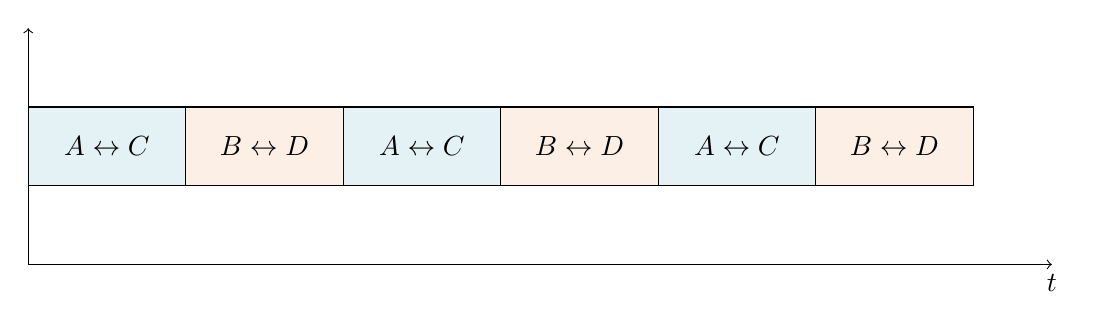
\begin{tikzpicture}
  \label{page:mux:tdm}

  \draw [->] (0,0) -- (0, 3); 
  \draw [->] (0,0) -- (13, 0);
  % \node [anchor=east] at (0,3) {$f$}; 
  \node [anchor=north] at (13,0) {$t$}; 

  \foreach \i in {0,4,8} {
    \draw [fill=hpiblue!10] (\i,1) -- ++(2,0) -- ++(0,1) -- ++(-2,0) -- ++(0,-1); 
    \node at (\i+1,1.5) {$A \leftrightarrow C$}; 
    \draw [fill=hpiorange!10] (\i+2,1) -- ++(2,0) -- ++(0,1) -- ++(-2,0) -- ++(0,-1); 
    \node at (\i+3,1.5) {$B \leftrightarrow D$}; 
  }
\end{tikzpicture}

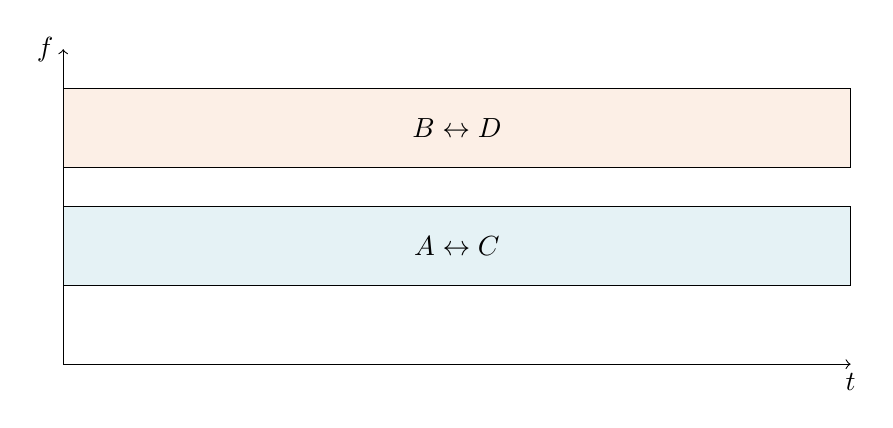
\begin{tikzpicture}
  \label{page:mux:fdm}

  \draw [->] (0,0) -- (0, 4); 
  \draw [->] (0,0) -- (10, 0);
  \node [anchor=east] at (0,4) {$f$}; 
  \node [anchor=north] at (10,0) {$t$}; 

  \draw [fill=hpiblue!10] (0,1) -- ++(10,0) -- ++(0,1) -- ++(-10,0) -- ++(0,-1); 
  \draw [fill=hpiorange!10] (0,2.5) -- ++(10,0) -- ++(0,1) -- ++(-10,0) --++(0,-1); 

  \node at (5,1.5) {$A \leftrightarrow C$}; 
  \node at (5,3) {$B \leftrightarrow D$}; 
\end{tikzpicture}


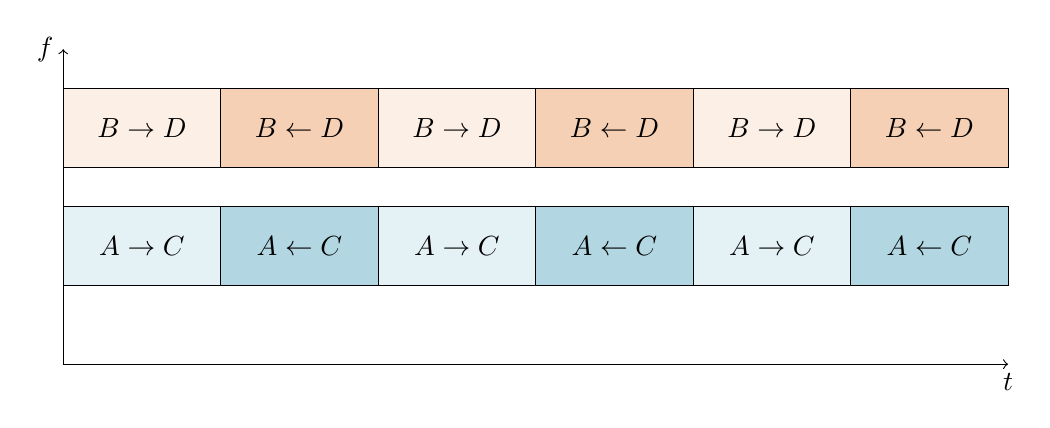
\begin{tikzpicture}
  \label{page:mux:fdm:tdd}

  \draw [->] (0,0) -- (0, 4); 
  \draw [->] (0,0) -- (12, 0);
  \node [anchor=east] at (0,4) {$f$}; 
  \node [anchor=north] at (12,0) {$t$}; 

  \foreach \i in {0,4,...,8} {
    \draw [fill=hpiblue!10] (\i,1) -- ++(2,0) -- ++(0,1) -- ++(-2,0) -- ++(0,-1); 
    \draw [fill=hpiblue!30] (\i+2,1) -- ++(2,0) -- ++(0,1) -- ++(-2,0) -- ++(0,-1); 
    \node at (\i+1,1.5) {$A \rightarrow C$}; 
    \node at (\i+3,1.5) {$A \leftarrow C$}; 
  }

  \foreach \i in {0,4,...,8} {
    \draw [fill=hpiorange!10] (\i,2.5) -- ++(2,0) -- ++(0,1) -- ++(-2,0) -- ++(0,-1); 
    \draw [fill=hpiorange!30] (\i+2,2.5) -- ++(2,0) -- ++(0,1) -- ++(-2,0) -- ++(0,-1); 
    \node at (\i+1,3) {$B \rightarrow D$}; 
    \node at (\i+3,3) {$B \leftarrow D$}; 
  }
  
\end{tikzpicture}


\end{document}